% Provenance (never printed): cycle 3 geography and "La planete Terre"
% (the great physical features of the world: relief, rivers, deserts, ice;
% reading a physical map); see sources/book1/PROVENANCE.md.
% Book 1, grade 4, chapter 3.
\chapter{La carte physique du monde}\label{ch:g4:world-physical-map}

Sami et Noor déplient une grande \omterm{def:g2:drawing-to-map:map}{carte} du monde sur le sol de la classe et
s'agenouillent autour. Elle ne ressemble pas aux \omterm{def:g2:drawing-to-map:map}{cartes} qu'ils connaissent.
Il n'y a ni pays, ni frontières, ni villes. À la place, les terres sont
peintes de couleurs~: vert le long des \omterm{def:g1:landscapes-around-us:water}{côtes} et dans les grandes étendues
plates, puis jaune pâle, puis brun, et à quelques endroits presque blanc.
La \omterm{def:g2:water-on-earth:ocean}{mer}, elle aussi, a plusieurs bleus~: pâle près des \omterm{def:g1:landscapes-around-us:water}{côtes}, de plus en
plus foncé au large, au milieu des \omterm{def:g2:water-on-earth:ocean}{océans}.

«~Pourquoi cette partie de l'Asie est-elle blanche~? demande Noor. C'est de
la \omterm{def:g4:clouds-rain-snow:precipitation}{neige}~?~» Pas tout à fait. Sur cette \omterm{def:g2:drawing-to-map:map}{carte}, chaque couleur dit à quelle
hauteur se trouvent les terres, ou à quelle profondeur est la \omterm{def:g2:water-on-earth:ocean}{mer}.

\begin{recall}
Une \omterm{def:g2:drawing-to-map:map}{carte} montre un lieu vu d'en haut, en plus petit~; sa \omterm{def:g2:drawing-to-map:legend}{légende} explique
ses couleurs et ses symboles (\cref{ch:g2:drawing-to-map}). Les terres
sont rassemblées en sept \omterm{def:g3:continents-and-oceans:continent}{continents}, entre cinq \omterm{def:g2:water-on-earth:ocean}{océans}, et un \omterm{def:g3:continents-and-oceans:world-map}{planisphère}
est un \omterm{def:g3:continents-and-oceans:globe}{globe} aplati (\cref{ch:g3:continents-and-oceans}). Les \omterm{def:g1:landscapes-around-us:landform}{montagnes},
les \omterm{def:g1:landscapes-around-us:landform}{collines}, les \omterm{def:g1:landscapes-around-us:landform}{vallées} et les \omterm{def:g1:landscapes-around-us:landform}{plaines} sont les \omterm{def:g1:landscapes-around-us:landform}{formes de relief}~; les
\omterm{def:g1:landscapes-around-us:water}{rivières} coulent des terres hautes jusqu'à la \omterm{def:g2:water-on-earth:ocean}{mer}
(\cref{ch:g1:landscapes-around-us}).
\end{recall}

\section{Lire une carte physique}

Pour dire à quelle hauteur se trouve un lieu, il nous faut un niveau de
départ, le même partout sur la Terre. Nous prenons le \omterm{def:g4:world-physical-map:altitude}{niveau de la mer}.

\begin{definition}[Altitude et niveau de la mer]\label{def:g4:world-physical-map:altitude}
Le \emph{niveau de la mer}\index{niveau de la mer} est le niveau moyen de la
surface de la \omterm{def:g2:water-on-earth:ocean}{mer}, entre la marée haute et la marée basse. L'\emph{altitude}\index{altitude}
d'un lieu est sa hauteur au-dessus du niveau de la \omterm{def:g2:water-on-earth:ocean}{mer}, en mètres. Sous la
\omterm{def:g2:water-on-earth:ocean}{mer}, on parle de \emph{profondeur}~: la distance qui sépare le fond de la
\omterm{def:g2:water-on-earth:ocean}{mer} du niveau de la \omterm{def:g2:water-on-earth:ocean}{mer}.
\end{definition}

Une ville au bord de la \omterm{def:g2:water-on-earth:ocean}{mer} a une \omterm{def:g4:world-physical-map:altitude}{altitude} de quelques mètres. Un village
de \omterm{def:g1:landscapes-around-us:landform}{montagne} peut se trouver à 1\,500 mètres~: un kilomètre et demi
au-dessus du \omterm{def:g4:world-physical-map:altitude}{niveau de la mer}, même s'il est à des centaines de kilomètres
de toute \omterm{def:g1:landscapes-around-us:water}{côte}.

\begin{definition}[Relief]\label{def:g4:world-physical-map:relief}
Le \emph{relief}\index{relief} d'une région est la forme de ses terres~: là
où elles sont hautes et là où elles sont basses, ses \omterm{def:g1:landscapes-around-us:landform}{montagnes}, ses
plateaux, ses \omterm{def:g1:landscapes-around-us:landform}{vallées} et ses \omterm{def:g1:landscapes-around-us:landform}{plaines}.
\end{definition}

\begin{definition}[Carte physique]\label{def:g4:world-physical-map:physical-map}
Une \emph{carte physique}\index{carte physique} montre le \omterm{def:g4:world-physical-map:relief}{relief} des terres
et la profondeur de la \omterm{def:g2:water-on-earth:ocean}{mer} par des couleurs, une couleur pour chaque palier
d'\omterm{def:g4:world-physical-map:altitude}{altitude} ou de profondeur, ainsi que les grands fleuves, les \omterm{def:g1:landscapes-around-us:water}{lacs}, les
déserts et les glaces.
\end{definition}

\begin{omfigure}
\begin{tikzpicture}
\begin{axis}[ommap, width=\linewidth, xtick=\empty, ytick=\empty, grid=none,
    axis background/.style={}, clip=true]
  \addplot graphics[xmin=-180, xmax=180, ymin=-90, ymax=90]
    {figdata/out/grade-4-physical_map.png};
  \addplot[black!45, line width=0.15pt] table {figdata/out/shared-geo-land.dat};
  \addplot[fill=omHypsSeaB, draw=blue!60!black, line width=0.2pt]
    table {figdata/out/grade-4-physical_map-lakes.dat};
  \addplot[blue!70!black, line width=0.5pt] table {figdata/out/grade-4-physical_map-rivers.dat};
  \begin{scope}[every node/.style={font=\scriptsize\bfseries, align=center,
      fill=white, fill opacity=0.7, text opacity=1, inner sep=1pt, rounded corners=1pt}]
    \node at (axis cs:-112,47) {Rocheuses};
    \node at (axis cs:-62,-22) {Andes};
    \node at (axis cs:10,49) {Alpes};
    \node at (axis cs:84,24) {Himalaya};
    \node at (axis cs:4,23) {Sahara};
    \node at (axis cs:-40,74) {Groenland\\(glace)};
    \node at (axis cs:60,-80) {Antarctique (glace)};
  \end{scope}
  \begin{scope}[every node/.style={font=\scriptsize\itshape, text=blue!50!black,
      fill=white, fill opacity=0.6, text opacity=1, inner sep=1pt}]
    \node at (axis cs:38,17) {Nil};
    \node at (axis cs:-56,-7) {Amazone};
    \node at (axis cs:-80,33) {Mississippi};
    \node at (axis cs:118,26) {Yangzi};
  \end{scope}
\end{axis}
\end{tikzpicture}

\smallskip
\begin{tikzpicture}[font=\scriptsize, x=1.18cm]
  \foreach \i/\c/\t in {0/5A9CCF/{plus de\\4000}, 1/84BCE0/{de 2000\\à 4000},
      2/B3D8EE/{de 200\\à 2000}, 3/DCEEF8/{de 0\\à 200}} {
    \definecolor{tmp}{HTML}{\c}
    \fill[tmp, draw=black!40] (\i,0) rectangle (\i+0.92,0.35);
    \node[align=center, anchor=north] at (\i+0.45,-0.05) {\t};
  }
  \foreach \i/\c/\t in {5/9CC98A/{de 0\\à 200}, 6/C9DE99/{de 200\\à 500},
      7/F1E7A8/{de 500\\à 1000}, 8/E5C58A/{de 1000\\à 2000}, 9/C79E76/{de 2000\\à 4000},
      10/ECE8E3/{plus de\\4000}} {
    \definecolor{tmp}{HTML}{\c}
    \fill[tmp, draw=black!40] (\i,0) rectangle (\i+0.92,0.35);
    \node[align=center, anchor=north] at (\i+0.45,-0.05) {\t};
  }
  \node[anchor=south] at (2,0.4) {profondeur de la mer (m)};
  \node[anchor=south] at (8,0.4) {altitude des terres (m)};
\end{tikzpicture}

{\small La \omterm{def:g4:world-physical-map:physical-map}{carte physique} du monde, avec sa \omterm{def:g2:drawing-to-map:legend}{légende}. Chaque couleur est un
palier d'\omterm{def:g4:world-physical-map:altitude}{altitude} (sur les terres) ou de profondeur (sous la \omterm{def:g2:water-on-earth:ocean}{mer}). Les
fleuves sont en bleu foncé. Le \omterm{def:g4:world-physical-map:relief}{relief} est dessiné à partir d'une valeur par
degré de latitude et de longitude (environ tous les 100 kilomètres)~: il
est donc lissé, et les sommets isolés comme les fosses étroites
n'apparaissent pas. Données~: \omterm{def:g4:world-physical-map:relief}{relief} NOAA ETOPO1~; fleuves, \omterm{def:g1:landscapes-around-us:water}{lacs} et
contours des côtes de Natural Earth.}
\label{fig:g4:world-physical-map:map}
% ledger: data:etopo1, data:b1-ne-rivers, data:ne-land
\end{omfigure}

\begin{method}[Lire une couleur sur une carte physique]\label{met:g4:world-physical-map:reading}
Pour trouver l'\omterm{def:g4:world-physical-map:altitude}{altitude} d'un lieu sur une \omterm{def:g4:world-physical-map:physical-map}{carte physique}~:
\begin{enumerate}
  \item trouve le lieu, et regarde sa couleur~;
  \item trouve la même couleur dans la \omterm{def:g2:drawing-to-map:legend}{légende}~;
  \item lis le palier écrit dessous~: l'\omterm{def:g4:world-physical-map:altitude}{altitude} du lieu est comprise entre
        les deux nombres.
\end{enumerate}
En \omterm{def:g2:water-on-earth:ocean}{mer}, on fait de même pour la profondeur.
\end{method}

\begin{example}[Trois lieux]\label{ex:g4:world-physical-map:three}
L'embouchure de l'Amazone, sur la \omterm{def:g1:landscapes-around-us:water}{côte} de l'Amérique du Sud, est vert
foncé~: son \omterm{def:g4:world-physical-map:altitude}{altitude} est comprise entre 0 et 200 mètres. Le centre du
Sahara est vert pâle ou jaune pâle~: entre 200 et 1\,000 mètres. Le plateau
au nord de l'Himalaya, en Asie, est presque blanc~: plus de 4\,000 mètres.
\end{example}

\section{Les grandes chaînes de montagnes}

Sur la \omterm{def:g2:drawing-to-map:map}{carte}, les couleurs brunes et blanches ne sont pas réparties
régulièrement. Elles forment de longues bandes étroites.

\begin{definition}[Chaîne de montagnes]\label{def:g4:world-physical-map:range}
Une \emph{chaîne de montagnes}\index{chaine de montagnes@chaîne de montagnes}
est une longue suite de \omterm{def:g1:landscapes-around-us:landform}{montagnes}, reliées entre elles, qui s'étend sur
des centaines ou des milliers de kilomètres.
\end{definition}

Les Andes longent tout le côté ouest de l'Amérique du Sud. L'Amérique du
Nord a les Rocheuses, l'Europe les Alpes, et l'Asie la plus haute de
toutes~: l'Himalaya. C'est là que se dresse la plus haute \omterm{def:g1:landscapes-around-us:landform}{montagne} de la
Terre~: l'Everest, haut de 8\,849 mètres, mesuré de nouveau en 2020.
% ledger: tht:everest

\begin{omfigure}
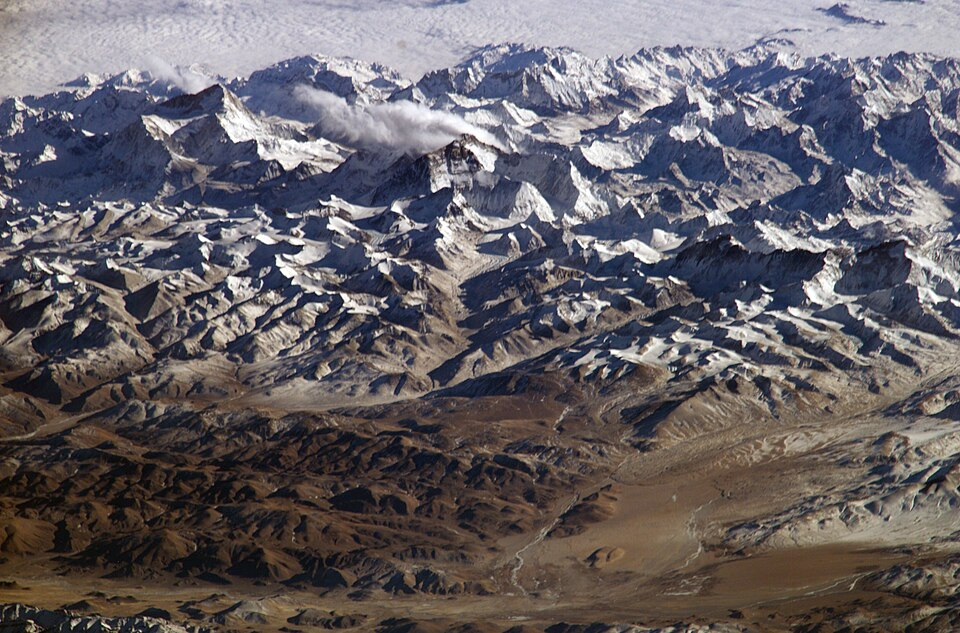
\includegraphics[width=0.75\linewidth]{images/book1/g4-himalaya-iss.jpg}

{\small L'Himalaya vu depuis la Station spatiale internationale, en
regardant vers le sud depuis le haut plateau du Tibet~: une \omterm{def:g2:water-on-earth:ocean}{mer} de sommets
enneigés. Photographie~: NASA (domaine public).}
% ledger: nasa:himalaya-iss
\end{omfigure}

\section{Les grands fleuves et les grands lacs}

La \omterm{def:g4:clouds-rain-snow:precipitation}{pluie} et la \omterm{def:g4:clouds-rain-snow:precipitation}{neige} fondue ruissellent sur les terres, se rassemblent en
ruisseaux puis en \omterm{def:g1:landscapes-around-us:water}{rivières}, et les \omterm{def:g1:landscapes-around-us:water}{rivières} emportent l'eau jusqu'à la \omterm{def:g2:water-on-earth:ocean}{mer}.
Les plus grands fleuves drainent des régions entières d'un \omterm{def:g3:continents-and-oceans:continent}{continent}.

Les deux plus longs fleuves de la Terre sont le Nil, en Afrique, et
l'Amazone, en Amérique du Sud. Chacun mesure près de 7\,000 kilomètres.
Lequel est le plus long~? Personne n'en est tout à fait sûr, car cela
dépend de l'endroit où l'on décide qu'un fleuve commence~: parmi tous les
petits ruisseaux qui se rejoignent pour le former, lequel compte comme son
vrai commencement~? En 2007, une équipe qui a remonté l'Amazone jusqu'à une
source plus lointaine a annoncé qu'il mesurait environ 6\,800 kilomètres,
un peu plus que le Nil~; beaucoup d'ouvrages de référence donnent
toujours le Nil comme le plus long.
% ledger: natgeo:nile, natgeo:amazon-nile-2007

L'Amazone est, sans aucun doute, le plus grand fleuve~: il transporte plus
d'eau que tous les autres.
% ledger: natgeo:amazon-nile-2007

\begin{omfigure}
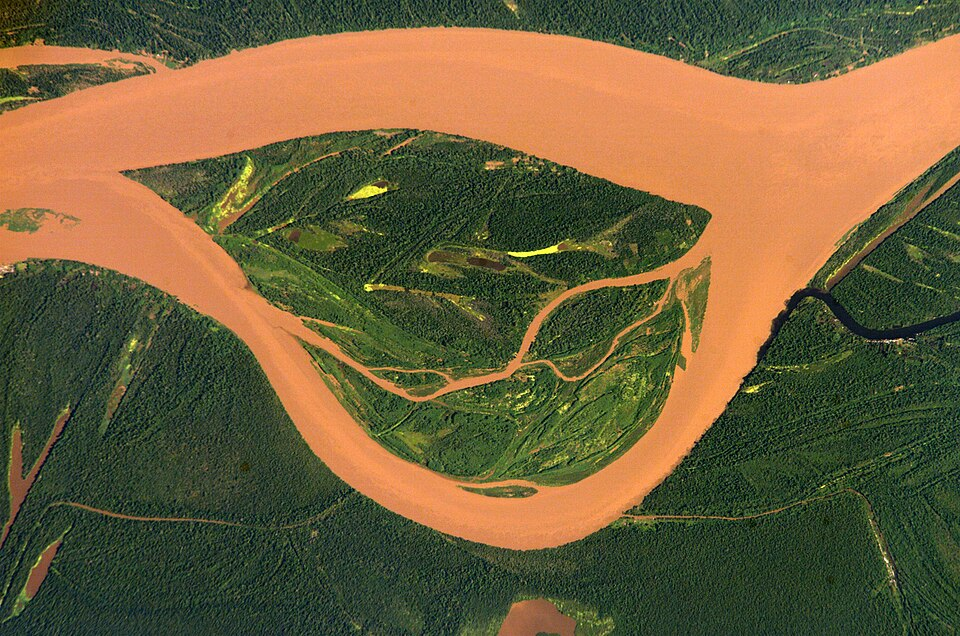
\includegraphics[width=0.6\linewidth]{images/book1/g4-amazon-iss.jpg}

{\small L'Amazone, brun de \omterm{def:g3:stones-pebbles-sand:sand}{boue}, serpentant à travers la forêt tropicale,
vu depuis la Station spatiale internationale. Photographie~: NASA (domaine
public).}
% ledger: nasa:amazon-iss
\end{omfigure}

Les \omterm{def:g1:landscapes-around-us:water}{lacs} battent aussi des records. Le plus grand \omterm{def:g1:landscapes-around-us:water}{lac} de la Terre est la
\omterm{def:g2:water-on-earth:ocean}{mer} Caspienne, entre l'Europe et l'Asie~: elle est si grande qu'on
l'appelle une \omterm{def:g2:water-on-earth:ocean}{mer}, mais elle est entourée de terres de tous les côtés.
Elle couvre plus de 370\,000 kilomètres carrés. Le \omterm{def:g1:landscapes-around-us:water}{lac} le plus profond est
le \omterm{def:g1:landscapes-around-us:water}{lac} Baïkal, en Russie~: par endroits, son fond se trouve à près de
2 kilomètres sous sa surface.
% ledger: natgeo:caspian-baikal

\section{Les déserts et les grandes glaces}

Deux sortes de lieux se remarquent sur la \omterm{def:g4:world-physical-map:physical-map}{carte physique}, parce que
presque rien n'y pousse~: les grands déserts, où il ne pleut presque
jamais, et les grandes glaces.

Le Sahara, dans le nord de l'Afrique, est le plus grand désert chaud de la
Terre. Il couvre environ huit millions et demi de kilomètres carrés.
L'Afrique tout entière couvre environ 30 millions de kilomètres carrés~: le
Sahara représente donc un peu plus du quart du \omterm{def:g3:continents-and-oceans:continent}{continent}~: plus de
$\frac{1}{4}$, mais moins de $\frac{1}{3}$.
% ledger: natgeo:sahara, data:etopo1

Les grandes glaces couvrent l'Antarctique, autour du \omterm{def:g3:continents-and-oceans:poles}{pôle Sud}, et la plus
grande partie du Groenland, tout au nord de l'Atlantique. Là, la \omterm{def:g4:clouds-rain-snow:precipitation}{neige} de
milliers d'années s'est accumulée et s'est changée en une épaisse couche
de glace. Sur la \omterm{def:g4:world-physical-map:physical-map}{carte physique}, ils ont les couleurs des terres hautes,
parce que le dessus de la glace est bien au-dessus du \omterm{def:g4:world-physical-map:altitude}{niveau de la mer}.

\section{Le plus haut et le plus profond}

La \omterm{def:g4:world-physical-map:physical-map}{carte physique} montre la forme de la surface de la Terre, mais elle est
si petite qu'elle cache les extrêmes. Mettons-les \omterm{def:g1:landscapes-around-us:water}{côte} à \omterm{def:g1:landscapes-around-us:water}{côte}, à l'échelle.

\begin{omfigure}
\begin{tikzpicture}[x=1cm, y=0.32cm, font=\small]
  % sea level
  \fill[omHypsSeaA] (0,0) rectangle (9,-11.5);
  \fill[omHypsSeaD!80] (4.6,-11.5) -- (4.6,-11.0) -- (5.0,-10.98) -- (5.4,-11.0) -- (5.4,-11.5) -- cycle;
  \draw[black!60] (-0.2,0) -- (9.2,0);
  \node[anchor=west, font=\scriptsize] at (9.25,0) {niveau de la mer, 0\,m};
  % height scale
  \draw[black!60] (0,-11.5) -- (0,10);
  \foreach \h in {-10,-8,...,8} {
    \draw[black!60] (-0.1,\h) -- (0,\h);
    \node[anchor=east, font=\scriptsize] at (-0.12,\h) {\h\,km};
  }
  % ocean floor and trench
  \fill[brown!45] (0.05,-11.5) -- (0.05,-3.7) -- (3.2,-3.7) -- (4.4,-6) -- (4.9,-10.98) -- (5.1,-10.98)
    -- (5.6,-6) -- (6.4,-3.7) -- (9,-3.7) -- (9,-11.5) -- cycle;
  \node[font=\scriptsize, align=center] at (2.0,-5.3) {fond de l'océan,\\environ 3\,700\,m};
  \node[font=\scriptsize, anchor=west, align=left] at (5.6,-9.4) {le point le plus profond~:\\l'abîme Challenger,\\près de 11\,000\,m};
  % Everest
  \fill[black!35] (6.6,0) -- (7.6,8.85) -- (8.6,0) -- cycle;
  \fill[white, draw=black!45, line width=0.3pt] (7.35,6.6) -- (7.6,8.85) -- (7.85,6.6) -- (7.6,7.1) -- cycle;
  \node[font=\scriptsize, align=center, anchor=south] at (7.6,8.95) {l'Everest, 8\,849\,m};
  % cirrus clouds band
  \draw[black!45, line width=0.6pt] (1.0,9.0) .. controls (1.6,9.5) and (2.2,9.1) .. (2.8,9.6);
  \draw[black!45, line width=0.6pt] (1.2,8.3) .. controls (1.8,8.8) and (2.4,8.4) .. (3.0,8.9);
  \node[font=\scriptsize, align=center] at (2.0,7.2) {nuages hauts\\(cirrus)};
  % a village
  \fill[black!60] (2.2,1.5) rectangle (2.45,1.75);
  \node[font=\scriptsize, anchor=west] at (2.5,1.6) {un village de montagne, 1\,500\,m};
\end{tikzpicture}

{\small Du point le plus profond de l'\omterm{def:g2:water-on-earth:ocean}{océan} au plus haut sommet, à
l'échelle. L'abîme Challenger, dans l'\omterm{def:g2:water-on-earth:ocean}{océan} Pacifique, est plus profond
sous la \omterm{def:g2:water-on-earth:ocean}{mer} que l'Everest n'est haut au-dessus d'elle. Valeurs~: l'Everest
8\,849\,m~; l'abîme Challenger près de 11\,000\,m~; le fond moyen de
l'\omterm{def:g2:water-on-earth:ocean}{océan} environ 3\,700\,m.}
\label{fig:g4:world-physical-map:extremes}
% ledger: tht:everest, usgs:trench-depth, nos:ocean-depth, wmo:cloud-levels
\end{omfigure}

\begin{example}[L'Everest au fond de l'abîme]\label{ex:g4:world-physical-map:everest-in-deep}
Si nous pouvions soulever l'Everest et le poser au fond de l'abîme
Challenger, son sommet serait encore sous l'eau~: environ 11\,000 mètres de
fosse, contre 8\,849 mètres de \omterm{def:g1:landscapes-around-us:landform}{montagne}. Plus de 2 kilomètres de \omterm{def:g2:water-on-earth:ocean}{mer} le
recouvriraient encore.
% ledger: tht:everest, usgs:trench-depth
\end{example}

\section{Exercices}

\begin{exercise}[$\star$]\label{exo:g4:world-physical-map:1}
Qu'est-ce que l'\omterm{def:g4:world-physical-map:altitude}{altitude} d'un lieu~? À partir de quel niveau la mesure-t-on~?
\end{exercise}

\begin{exercise}[$\star$]\label{exo:g4:world-physical-map:2}
À l'aide de la \omterm{def:g2:drawing-to-map:legend}{légende} de la \omterm{def:g4:world-physical-map:physical-map}{carte physique}, donne l'\omterm{def:g4:world-physical-map:altitude}{altitude} d'un lieu
colorié~: (a) en vert foncé~; (b) en jaune pâle~; (c) presque en blanc.
\end{exercise}

\begin{exercise}[$\star$]\label{exo:g4:world-physical-map:3}
Sur quel \omterm{def:g3:continents-and-oceans:continent}{continent} se trouvent~: (a) les Andes~; (b) l'Himalaya~; (c) le
Sahara~; (d) les Rocheuses~?
\end{exercise}

\begin{exercise}[$\star$]\label{exo:g4:world-physical-map:4}
Nomme la plus haute \omterm{def:g1:landscapes-around-us:landform}{montagne} de la Terre, le plus grand \omterm{def:g1:landscapes-around-us:water}{lac} et le \omterm{def:g1:landscapes-around-us:water}{lac} le plus profond.
\end{exercise}

\begin{exercise}[$\star$]\label{exo:g4:world-physical-map:5}
Sur la \omterm{def:g4:world-physical-map:physical-map}{carte physique}, la \omterm{def:g2:water-on-earth:ocean}{mer} près des \omterm{def:g1:landscapes-around-us:water}{côtes} est bleu pâle et le milieu des
\omterm{def:g2:water-on-earth:ocean}{océans} bleu foncé. Qu'est-ce que cela t'apprend sur la profondeur de la \omterm{def:g2:water-on-earth:ocean}{mer}~?
\end{exercise}

\begin{exercise}[$\star$]\label{exo:g4:world-physical-map:6}
Pourquoi l'Antarctique et le Groenland ont-ils la couleur des terres hautes
sur la \omterm{def:g4:world-physical-map:physical-map}{carte physique}~?
\end{exercise}

\begin{exercise}[$\star\star$]\label{exo:g4:world-physical-map:7}
Range du plus bas au plus haut~: une plage~; un village à 1\,500 mètres~;
le sommet de l'Everest~; le fond de l'abîme Challenger~; le fond moyen de
l'\omterm{def:g2:water-on-earth:ocean}{océan}.
\end{exercise}

\begin{exercise}[$\star\star$]\label{exo:g4:world-physical-map:8}
Pourquoi ne peut-on pas dire avec certitude si c'est le Nil ou l'Amazone
qui est le plus long fleuve~?
\end{exercise}

\begin{exercise}[$\star\star$]\label{exo:g4:world-physical-map:9}
L'Afrique couvre environ 30 millions de kilomètres carrés. Combien fait le
quart~? Le tiers~? Le Sahara couvre environ huit millions et demi de
kilomètres carrés~: est-ce plus ou moins que le quart de l'Afrique~? Plus
ou moins que le tiers~?
\end{exercise}

\begin{exercise}[$\star\star$]\label{exo:g4:world-physical-map:10}
Un refuge de \omterm{def:g1:landscapes-around-us:landform}{montagne} se trouve à 2\,500 mètres, et un \omterm{def:g1:landscapes-around-us:water}{lac} en contrebas à
1\,000 mètres. De combien de mètres le refuge est-il plus haut~? Quelles
couleurs ont-ils sur la \omterm{def:g4:world-physical-map:physical-map}{carte physique}~?
\end{exercise}

\begin{exercise}[$\star\star\star$]\label{exo:g4:world-physical-map:11}
Un avion vole à 10 kilomètres au-dessus du \omterm{def:g4:world-physical-map:altitude}{niveau de la mer}. Est-il plus
haut que l'Everest~? De combien de mètres~? S'il survolait l'abîme
Challenger, à quelle distance du fond de la fosse serait-il (prends
11\,000 mètres pour la fosse)~?
\end{exercise}
